% Created 2021-03-28 dim. 17:11
% Intended LaTeX compiler: pdflatex
\documentclass[a4paper,12pt]{article}
\usepackage[position=top,labelformat=empty]{subfig}
\usepackage{caption}
\usepackage[hmargin=2cm,vmargin=3cm]{geometry}


\usepackage{amsmath}
\usepackage{caption,graphicx,subcaption}
\usepackage[boxed]{algorithm2e}
\usepackage{authblk}
\author[1]{Vaitea Opuu}
\author[1]{Nono S. C. Merleau}
\author[1]{Matteo Smerlak}
\affil[1]{Max Planck Institute for Mathematics in the Sciences, D-04103 Leipzig, Germany}
\date{\today}
\title{A Mirror encoding combined with the FFT for a fast heuristic of the RNA folding dynamics}
\begin{document}

\maketitle

\section{Abstract}
\label{sec:org03f64b1}
\begin{itemize}
\item Simple and fast heuristic for the folding path of RNAs.
\item It is straightforward to model Pseudoknots
\item It's performance is comparable to exact method on the RNA folding problem
\item It follows a simple idea which naively corresponds to RNA folds mechanism
(many BPs formed at once to compensate for the lost of entropy)
\item Among the 50 predicted structures, in average, at least one has pvv \textasciitilde{} 74\% and
sensitivity \textasciitilde{} 76\%.
\item We propose a fast algorithm method based on the FFT to search for high density
BP regions.
\item There are smooth coarse-grain folding path which lead to near native structures.
\end{itemize}

\clearpage
\section{Introduction}
\label{sec:org614aaae}
\subsection{RNA folding introduction}
\label{sec:org8769818}
bla bla dynamic of secondary structure relevant bla biological function.

\begin{itemize}
\item MFE and MEA not significantly different in term of performances (how to bench RNA)
\end{itemize}

\subsection{RNA folding dynamics}
\label{sec:orgbcb036b}
\begin{enumerate}
\item Description of RNA structure
\item going up to the 2ndary structure only
\item Simple rules to compute a structure: multiple BPs compensate the lost of
entropy during the folding process.
\end{enumerate}
\subsection{Energy model}
\label{sec:org0ce990e}
\begin{enumerate}
\item issue with additivity principle in model. Might be worst when the sequence
lengthens since more tertiary interactions interplay.
\end{enumerate}
\subsection{Existing methods}
\label{sec:orgb299693}
\begin{enumerate}
\item MC sampling: kinefold; atomic moves; MC-style simulation
\item Barrier trees from conformation landscape subopt tree: Sample from the
boltzmann ensemble of structures
\item Vfold, simplified folding model
\end{enumerate}

\clearpage
\section{FFT based folding dynamic heuristic}
\label{sec:org47bec4d}
We now describe the heuristic folding algorithm starting from one sequence S and
its associated unfolded structure of lenght L. We first create a numerical
representation of S where each type of nucleotide in replaced by a unit vector
of 4 components:
\begin{equation}
\begin{split}
A \rightarrow \begin{pmatrix} 1 0 0 0 \end{pmatrix}
U \rightarrow \begin{pmatrix} 0 0 0 1 \end{pmatrix}
C \rightarrow \begin{pmatrix} 0 1 0 0 \end{pmatrix}
G \rightarrow \begin{pmatrix} 0 0 1 0 \end{pmatrix}
\end{split}
\end{equation}
which gives us a \(4 \times L\) matrix we call X where each row is a nucleotide
type channel. Here, the first row would be the A channel which we refer to as
\(X^A\). Then, we create a second copy for which we revert the order of the
sequence and use the following complementary encoding:
\begin{equation}
\begin{split}
\bar{A} \rightarrow \begin{pmatrix} 0 0 0 w_{\scalebox{0.5}{AU}} \end{pmatrix}
\bar{U} \rightarrow \begin{pmatrix} w_{\scalebox{0.5}{AU}} w_{\scalebox{0.5}{GU}} 0 0 \end{pmatrix}
\bar{C} \rightarrow \begin{pmatrix} 0 0 w_{\scalebox{0.5}{GC}} 0 \end{pmatrix}
\bar{G} \rightarrow \begin{pmatrix} 0 w_{\scalebox{0.5}{GC}} 0 w_{\scalebox{0.5}{GU}} \end{pmatrix}
\end{split}
\end{equation}
where \(w_{AU}\), \(w_{GC}\), \(w_{GU\) are tunable parameters for the next step. We
call this new copy \bar{X}, the mirror of X.

For each of the 4 components, we compute the correlation between X and \bar{X}
and simply sum up the four channels to obtain the correlation between the two
copies:
\begin{equation}
cor(k) = (c_{X^A,\bar{X}^A}(k) + c_{X^U,\bar{X}^U}(k) + c_{X^G,\bar{X}^G}(k) + c_{X^C,\bar{X}^C}(k)) / min(k, 2 \times L-k)
\end{equation}
where \(c_{X^A,\bar{X}^A(k)\) is the correlation in the \(A\) channel between the
two copies. The correlation \(cor(k)\) gives the average number of base pairs for
a positional lag \(k\). One channel correlation between the copies is given by:
\begin{equation}
c_{X^A,\bar{X}^A}(k) = \sum\limits_{1\leq i \leq L, 1 \leq i + k \leq M} X^A(i) \times \bar{X}^A(i+k)
\end{equation}
where \(X^A(i)\) and \(\bar{X}^A(i+k)\) are the A channel of site \(i\) and \(i+k\).
X\textsuperscript{A}(i) \texttimes{} \bar{X}\textsuperscript{A}(i+k) is non zero if sites \(i\) and \(i+k\) can form a base
pair, and will be the value of the chosen weight as described above. Although
this operation requires \(O(N^2)\) operation, it can take advantage of the FFT
which reduces drastically its complexity to \(O(Nlog(N))\).

The large correlation values between the two copies indicates the positional lag
between at which the base pair density is high. Therefore, we use a sliding
window strategy to search for the longest consecutive base pairs within the
positional lag. Since the copies are symmetrical, we only need to slide over one
half of the positional lag. Once the longest base pairs are identified, we
simply compute the free energy change when those base pair are formed. We
perform the same search for the \(n\) highest correlation lags, which gives us \(n\)
possible possibilities. Then, we added to the current structure the base pairs
that gives the best change of energy.

We are now left with two segments, the interior and exterior of the group of
consecutive base pairs formed. The two exterior fragments are concatenated
together. Then, we simply apply recursively the same procedure on the two
segments separately in a "Breath First" fashion to form new consecutive base
pairs, until no base pair formation can improve the energy. However, it is
straightforward to consider pseudoknots by simply concatenating all the
fragments left.

The algorithm described so far tends to be stuck in the first local minima found
along the folding trajectory. To alleviate this, we propose a stacking procedure
where the 50 best trajectories are stored in a stack and evolved in parallel.
Hence, it offers the flexibility of overcoming some energy barriers. \textbf{Figure}
shows the whole procedure.

\section{Folding RNAs}
\label{sec:orga1ab6cf}
To evaluate the relevance of the folding model, we compared the algorithm
performance for the folding task. In addition, to assess the effect of sequence
lengthens on these predictions, we displayed their performance length-wise.

\textbf{Figure} shows the performance in PPV and sensitivity for the four methods. It
shows that the ML method is consistently better than thermodynamic methods.
Length-wise T-test between the MFE and ML predicitons showed that this
difference is significant (pvalue \(\approx\) 10\textsuperscript{-12}) with a substantial
improvement of about 10\%. Although RAFFT predictions were found to be comparable
to MFE predictions, they are significantly less accurate (pvalue \(\approx\)
0.0002), with a drastic lost of performance for sequences of length greater than
300 nucleotides.

Among the 50 configurations produced by RAFFT, we found in average at least one
prediction with in average 59\% of PPV and <SENS> of sensitivity (blue curve in
\textbf{figure}). The overall gain of performances is not significantly different from
the MFE predictions. However, for the sequences of length lesser than 200
nucleotides, this gain was found to be substantial and significant (\(\approx\) 16 \%
better than the MFE). The accuracy for those sequences is equivalent to ML
performances. For sequence lengths greater than 300 nucleotides, we observed the
same drastic lost of accuracy, although we took only the best prediction among
the 50 saved configurations for each sequence.

Two regions of lack of performances were observed for all methods. A group of 28
sequences of length shorter than 80 nucleotides were evaluated with free of
their known structures about 9.8 kcal/mol greater than the MFE structures. Some
of them involve large exterior loop such as displayed in \textbf{figure}. The second
region is around 200 nucleotides length. The known structure of these sequences
also displayed large unpaired regions such as the one shown in \textbf{figure}.

\begin{figure}[htbp]
\centering
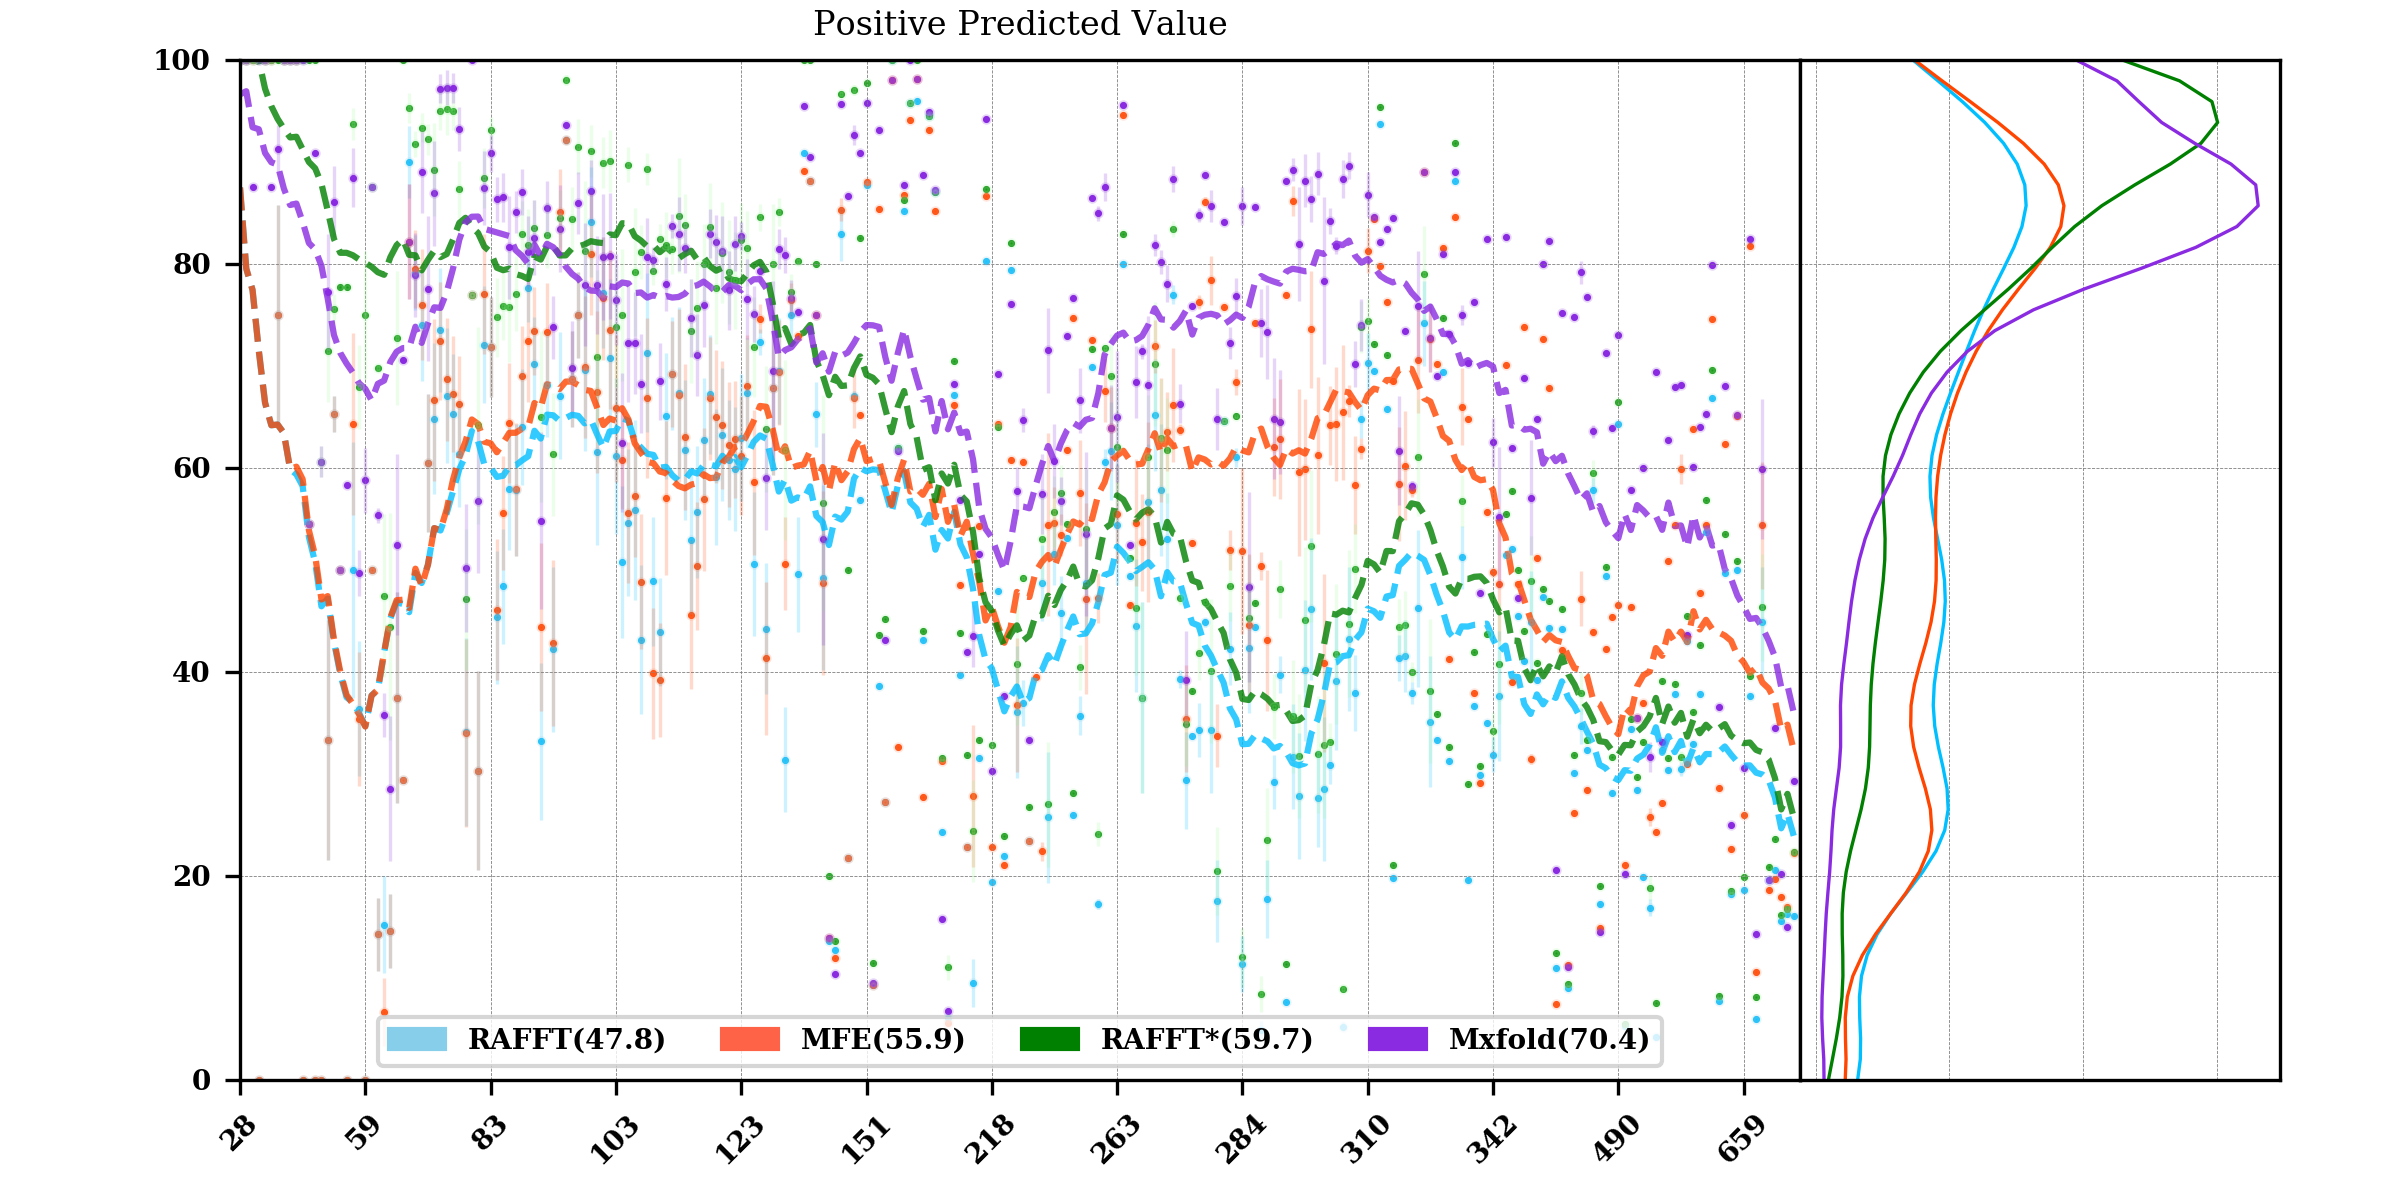
\includegraphics[width=.9\linewidth]{img/fold_perf_pvv.png}
\caption{Folding comparison by taking the best energy among the 30 predicted trajectories}
\end{figure}

To investigate the region of the structure space where the thermodynamic model
tends to fail, we computed the composition content of the known structures.
\textbf{Figure} shows the prcent of base pairs or positions involved in the five loop
types: interior, exterior, hairpin, stacking, and multi-branch loops. Those
prcents were then represented in a principal component analysis. From the PCA,
we observed that the known structures are distributed in the structure space
non-uniformly. Some natural structures, as observed above, have large exterior
loops. The center of mass in the principal component space is located in between
the high density stacking and interior loops. This shows that the dataset
contains many elongated structures.

It shows that the MFE predictions tend to fail when the structure contains a
high proportion of interior loops as shown in \textbf{figure}.

\begin{figure}[htbp]
\centering
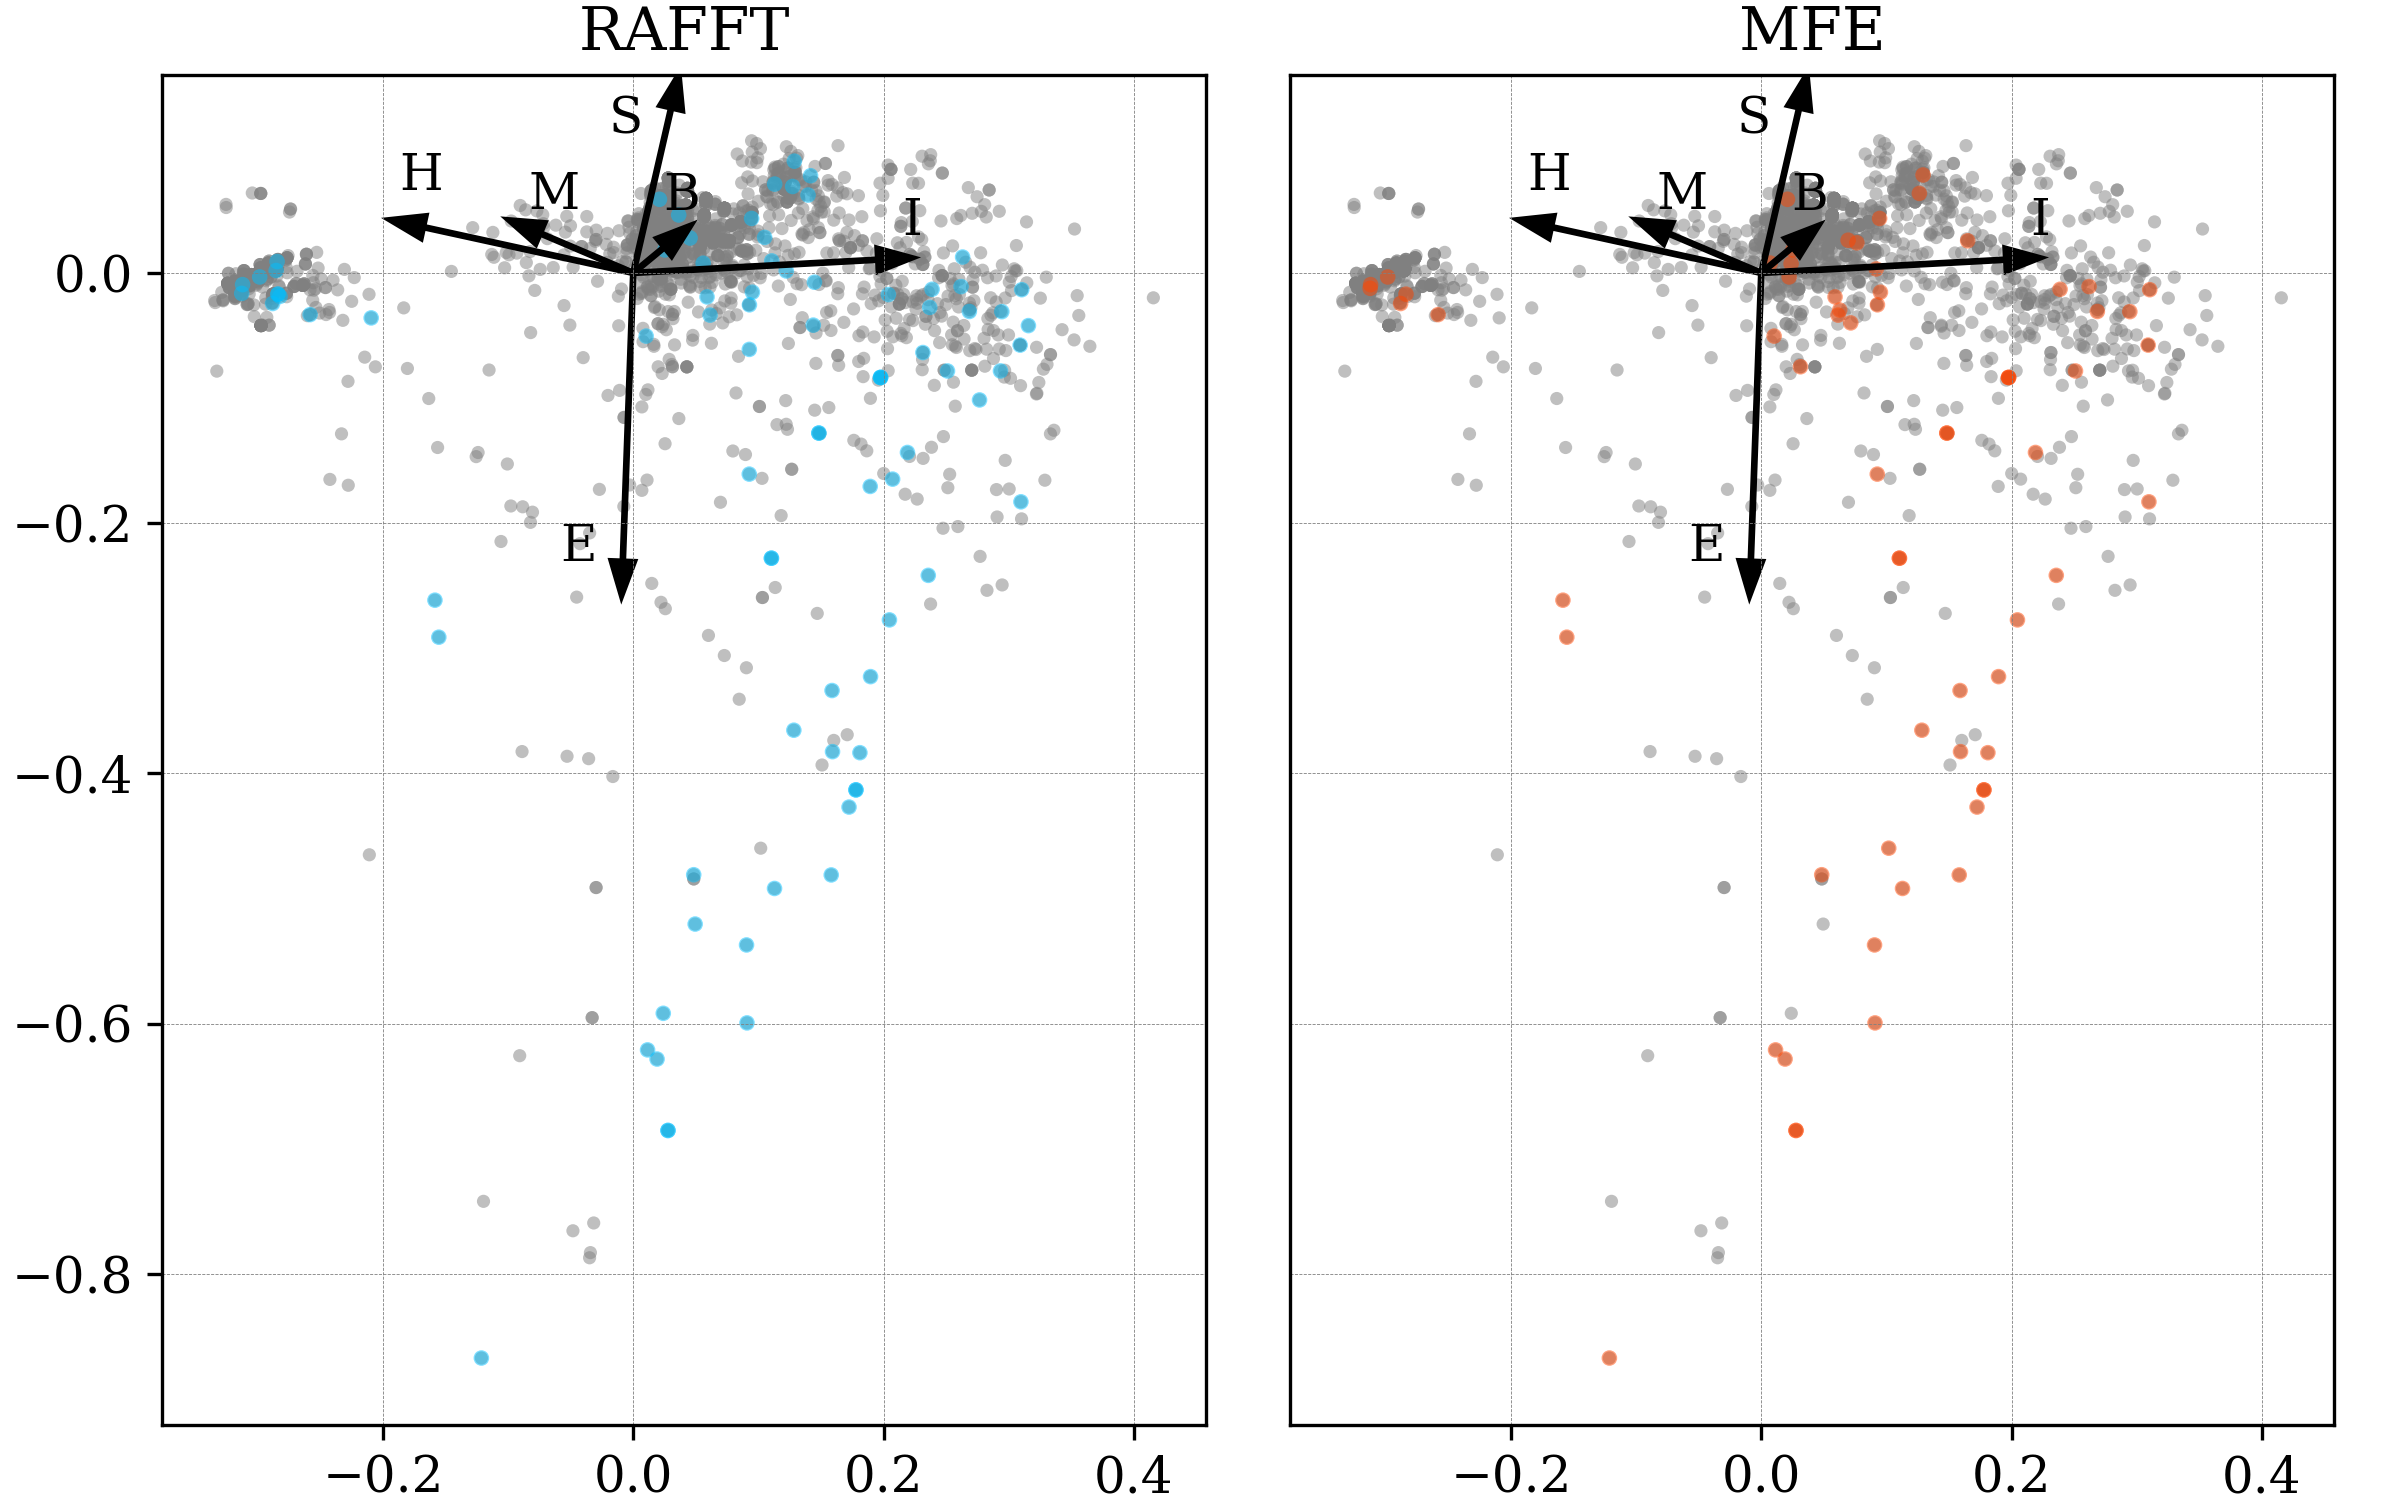
\includegraphics[width=.9\linewidth]{img/comp_fails.png}
\caption{where does the methods failed? PCA RNAfold, Mxfold, FFT, and}
\end{figure}

\begin{figure}[htbp]
\centering
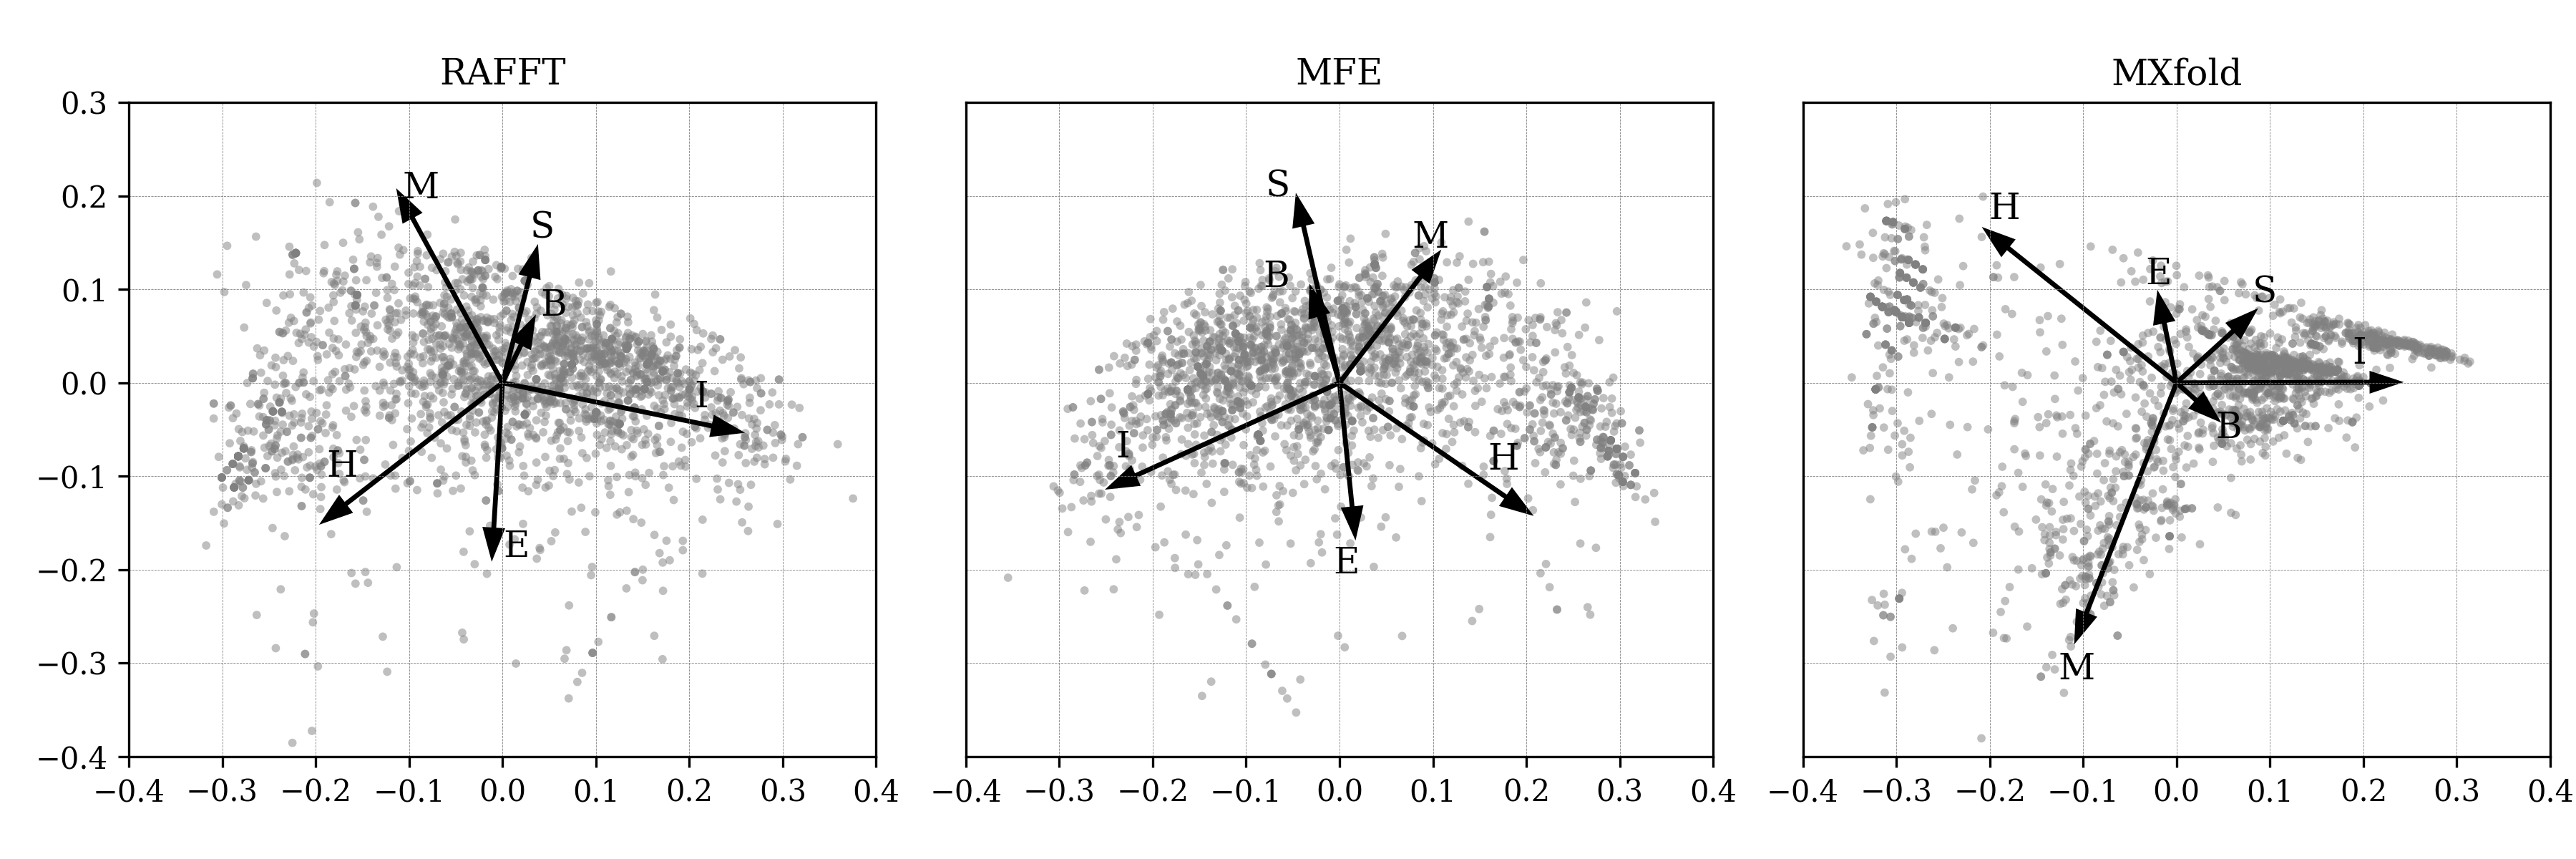
\includegraphics[width=.9\linewidth]{img/content_predicted_data.png}
\caption{What kind of structure these method naturally produce}
\end{figure}

\section{Methods}
\label{sec:orga61564e}
We formed two sub-datasets based on the ArchiveII (\textbf{ref}) dataset. First, we
removed from all the structure containing pseudoknot since all tool considered
here don't handle pseudoknots. Next, we removed all the structures which were
evaluated with a positive energy or null energy with the Turner 2004 energy
parameters. Since positive energies means that the completely unfolded structure
is more stable than the native one, we assume that those structures are not well
modeled by the energy function used here. This dataset is composed of 2698
structures. 240 sequences were found multiple times (from 2 to 8 times). 19 of
them were found with different structures. We discarded all duplication and
picked the structure with the lowest energy for each. We obtained a dataset of
2296 sequences.

To compute the MFE structure, we used RNAfold (version) with the default
parameters and the Turner 2004 set of energy parameters. For the machine
learning tool, we computed the prediction using Mxfold2 with the default
parameters. The structures for both were used for the statistics.

For kinfold, we performed for each sequence, 40 simulations of 10\textsuperscript{4} (unit?).
Then, we counted the occurrences of each structures and selected the 50 most
populated structures. The best structure in terms of PPV was displayed and used
for the statistics.

For the FFT-based algorithm, we used two sets of parameters. First, we used
search for consecutive base pairs in the 50 best modes and stored 50
conformations for which we displayed the best energy found. The correlation were
computed using the weights w\textsubscript{GC}=3, w\textsubscript{AU}=2, and w\textsubscript{GU}=1.

To measure the predictions accuracy, we used two metrics from epimiology. The
positive predictive value (PPV) which is the fraction of correct base pairs
predictions in the predicted structure. The sensitivity is the fraction of
correctly predicted base pairs in the true structure. Both metrics are defined
as follow:
\begin{equation}
PPV = \frac{TP}{TP + FN} \;\;\; \text{Sensitivity} = \frac{TP}{TP+FP}
\end{equation}
where TP, FN, and FP stand respectively for the number of correctly predicted
base pairs (true positives), the number of base pairs not detected (false
negatives), and the number of wrongly predicted base pairs (false positives). To
maintain consistency with previous and future studies, we computed these metrics
using the implementation in the \texttt{scorer} tool provided in \textbf{ref Mathews}, which
provide also a more flexible estimate where shift are allowed.

The loop composition were extracted in terms of proportion to have an overall
measure of the structure distribution. We first convert all natural structures
into Shapiro notation using Vienna Package utilies. From the notation, we
extracted the proportion of base pairs involved into the interior, exterior,
bulge, stacking, and multibranch loops. For each true structure, we obtained a
prcent of type of loops from which we extracted the principal components. Next,
the structure compositions where projected on the first two principal components
for visual conveniences. The composition arrows represents the eigen vectors
obtained from the diagonalization of the covariance matrix.

\clearpage
\section{Concluding discussion}
\label{sec:org66df435}
\subsection{Good stuff}
\label{sec:org31cbbc4}
\begin{enumerate}
\item Simple heuristic to compute folding path
\item Versatile method: allow simple modeling of pseudoknot and more information
can be encoded in the mirror representation.
\item Performance is comparable although not as good as state of the art in the
folding task.
\item One trajectory among the selected produce good structures (close with better
accuracy than ML methods).
\end{enumerate}

\subsection{limits}
\label{sec:orgf0917bf}
\begin{enumerate}
\item Choosing the maximum number each time is not an optimal choice
\item In average, the scores are not good. Only a few out of the predicted
structures have good scores.
\item The quality of the prediction degrade drastically when the size > 250 from
74\% -> 50\%.
\begin{enumerate}
\item The stacking method might one cause however, since MFE is degraded as
well, we believe that it might partly explain by the thermodynamic model
accuracy.
\end{enumerate}
\item The distribution of loop types composition seems to differ between the
Boltzmann ensemble and the natural structures.
\end{enumerate}
\end{document}
